\chapter{Objetivos}
El proyecto se basa en el diseño, fabricación y caracterización de un biosensor electroquímico sobre un sustrato flexible a ser utilizado en la plataforma NanoPoc (Figura ~\ref{fig:Figura_Nano_Poc}), desarrollada en el Instituto Nacional de Tecnología Industrial, para la detección de enfermedades bacterianas, virales o parasitarias en salud humana y sanidad animal \cite{PosterPoc2}.

\begin{figure}[H]
  \centering
    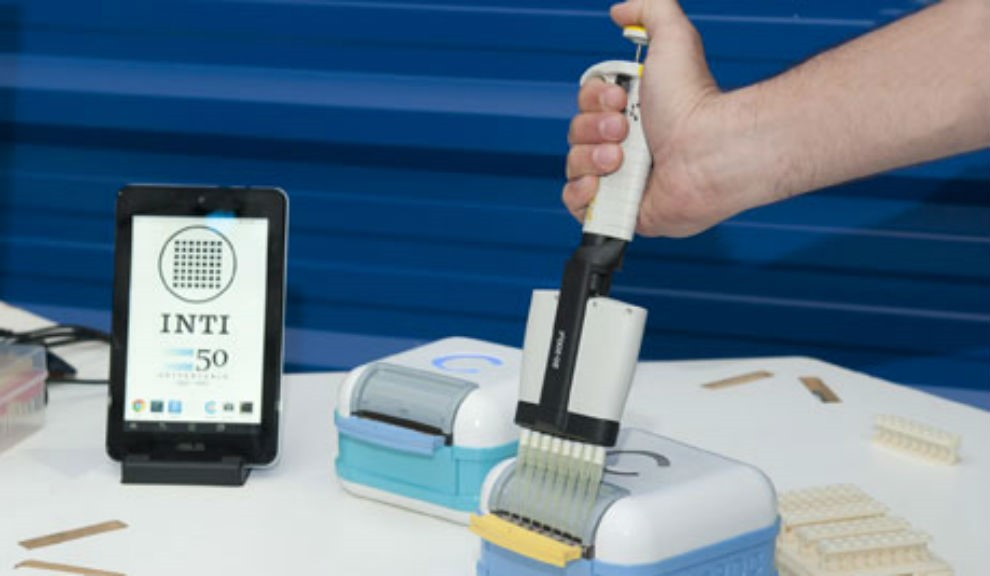
\includegraphics[width=0.5\textwidth]{Figuras/Figura_Nano_Poc}
  \caption{Plataforma NanoPoc.}
  \label{fig:Figura_Nano_Poc}
\end{figure}

\section{Objetivos Generales}
El objetivo principal es generar un biosensor de fácil fabricación y con alta reproducibilidad. Se pretende mejorar el uso del mismo, evitando el manejo de preparación de muestras entre la extracción y la medición en el dispositivo, para la detección $``$\textit{in situ}$"$ de enfermedades infecciosas en humanos y animales, dependiendo del tipo de biorreceptor desarrollado (Figura ~\ref{fig:Figura_Biosensor_objetivos}).
\begin{figure}[H]
  \centering
    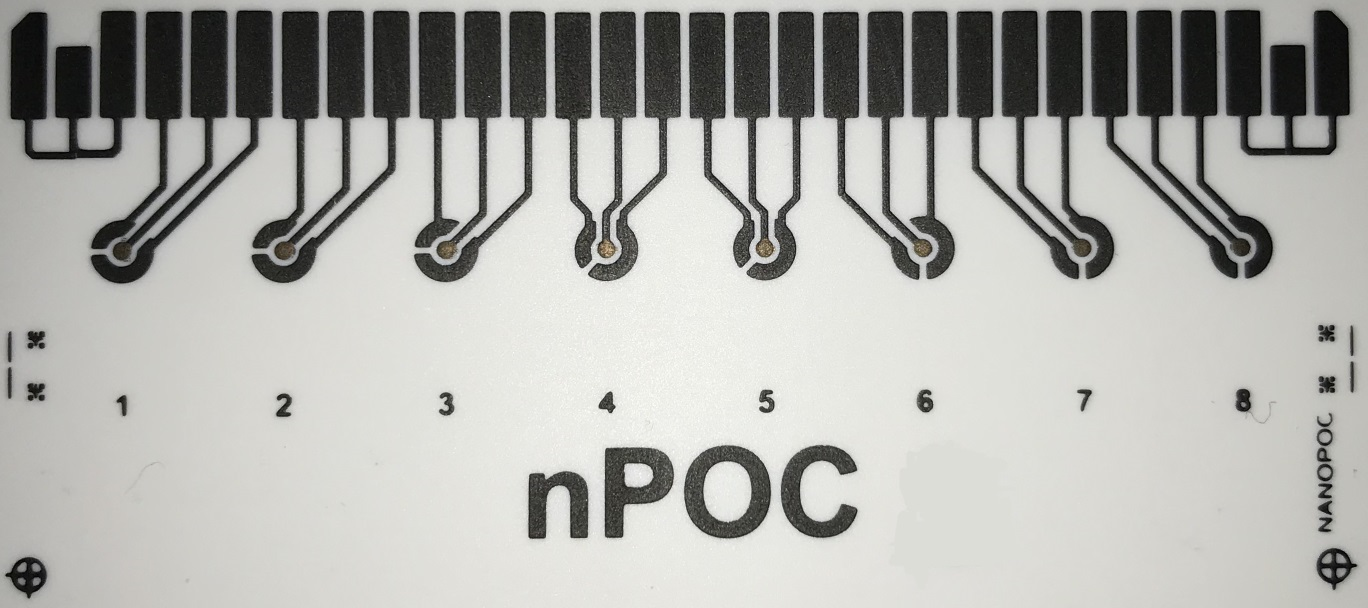
\includegraphics[width=0.5\textwidth]{Figuras/Figura_Biosensor_objetivos}
  \caption{Biosensor.}
  \label{fig:Figura_Biosensor_objetivos}
\end{figure}
\section{Objetivos Espec\'ificos}
- Fabricar los sensores con la forma adecuada, mediante una deposición controlada de material sobre el sustrato flexible, creando 8 celdas electroquímicas con las dimensiones estándar de una micropipeta de 8 canales (Figura ~\ref{fig:Figura_celda_electroquimica}).\\
\begin{figure}[H]
  \centering
    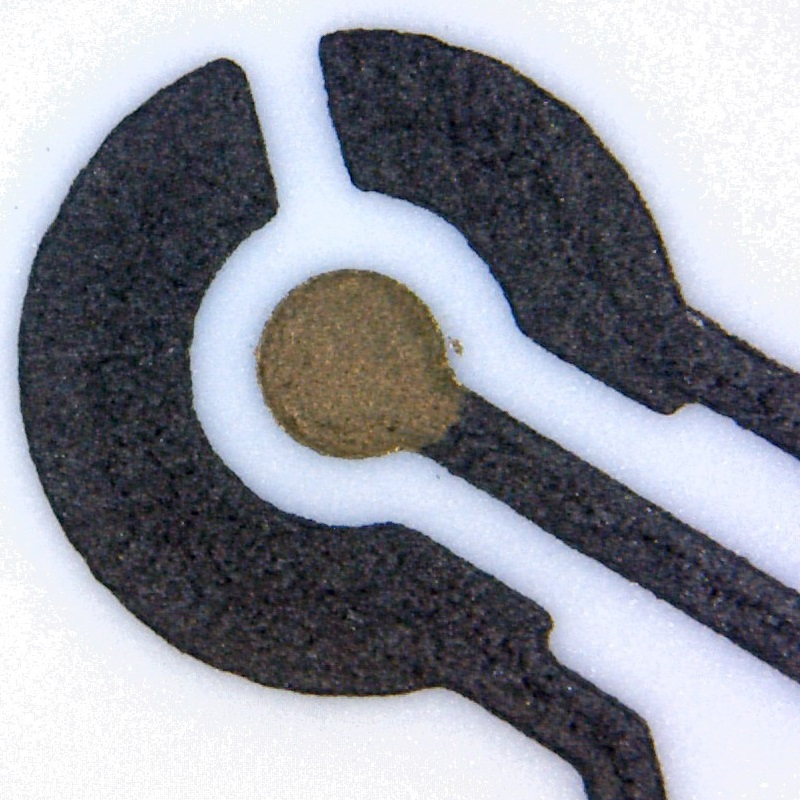
\includegraphics[width=0.35\textwidth]{Figuras/Figura_celda_electroquimica}
  \caption{Celda electroquímica.}
  \label{fig:Figura_celda_electroquimica}
\end{figure}
- Calibrar la impresora \textit{inkjet} con el fin de obtener el diseño del biosensor deseado utilizando una tinta específica sobre el sustrato elegido (Figura ~\ref{fig:Figura_impresora_objetivos}).\\
\begin{figure}[H]
  \centering
    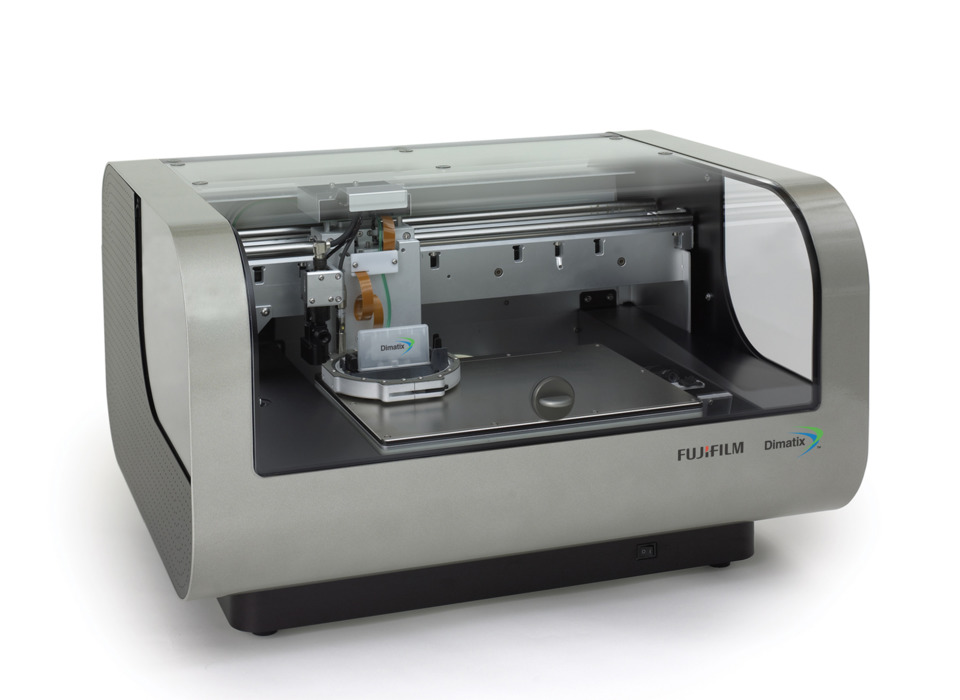
\includegraphics[width=0.5\textwidth]{Figuras/Figura_impresora_objetivos}
  \caption{Impresora \textit{Inkjet}.}
  \label{fig:Figura_impresora_objetivos}
\end{figure}
- Obtener una respuesta correcta de los biosensores mediante una solución química equivalente a un analito específico utilizando la técnica electroquímica del tipo amperométrico (Figura ~\ref{fig:Figura_caracElectroquim_objetivos}).\\
\begin{figure}[H]
  \centering
    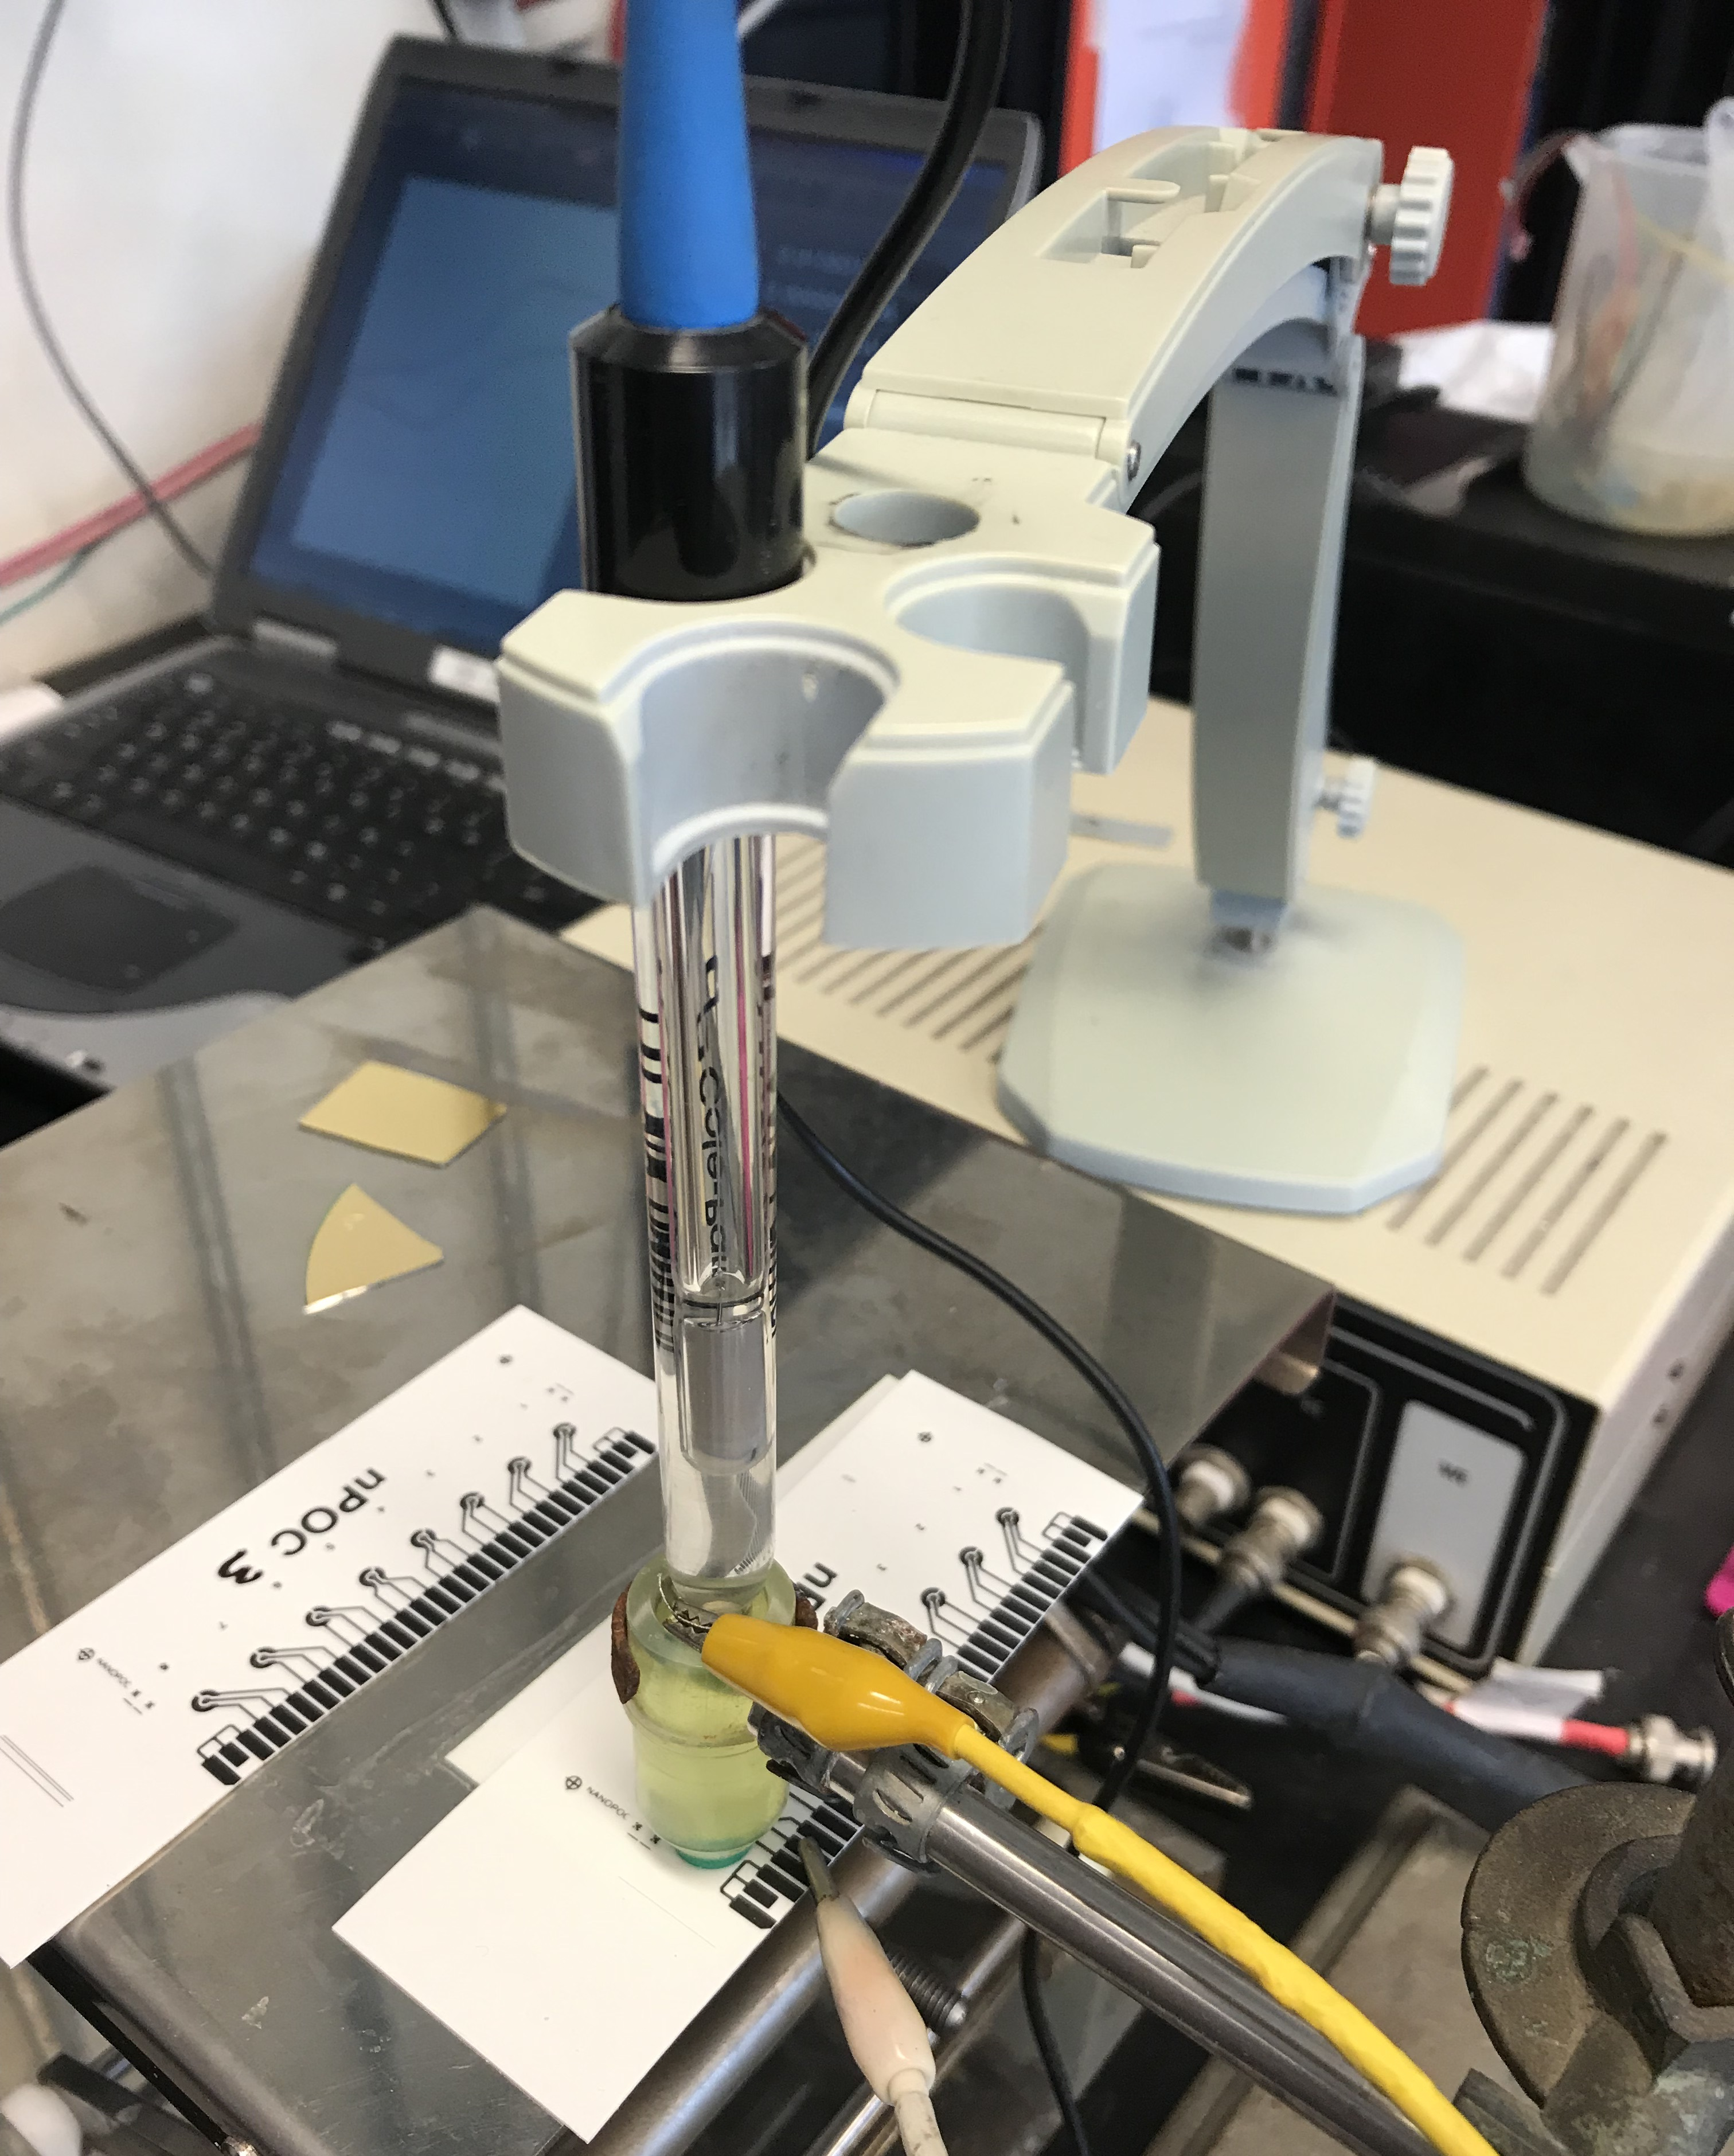
\includegraphics[width=0.4\textwidth]{Figuras/Figura_caracElectroquim_objetivos}
  \caption{Caracterización electroquímica.}
  \label{fig:Figura_caracElectroquim_objetivos}
\end{figure}